\subsection{Dependency Probing (RQ4)}
\label{sec:rq4}

\begin{figure}[t]
 	\centering
 	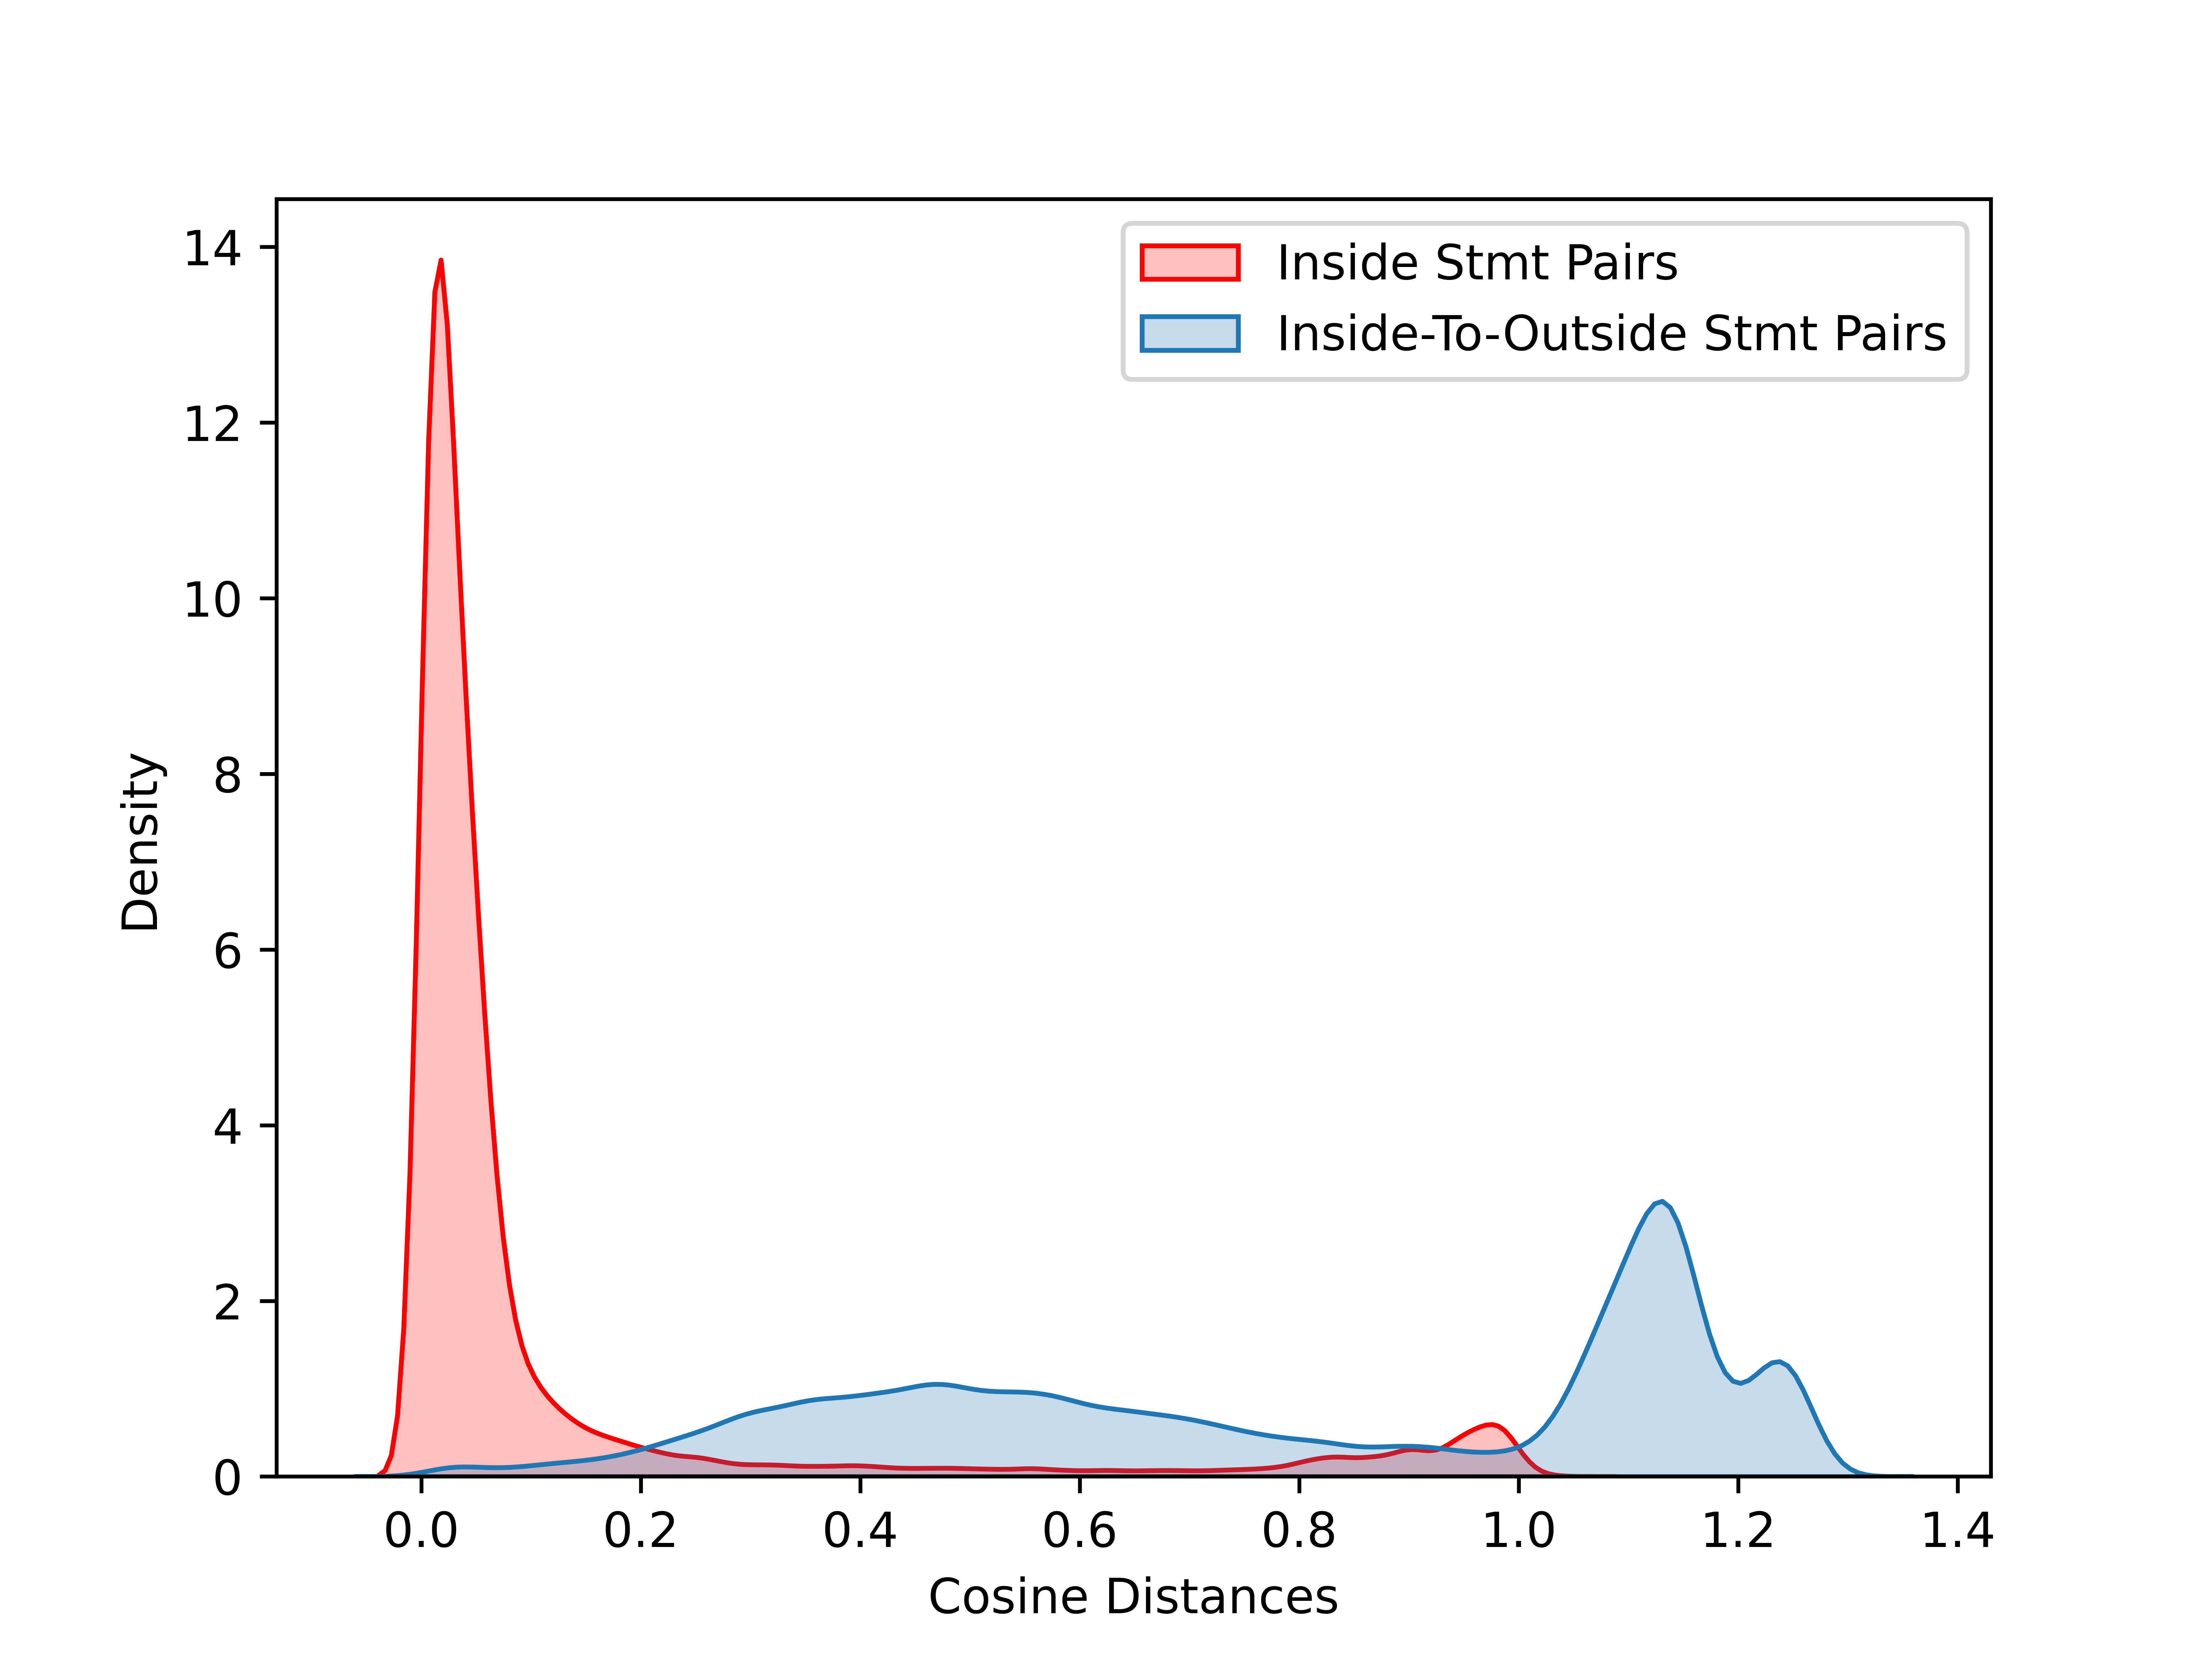
\includegraphics[width=3.4in]{rq4-density.png}
        \vspace{-20pt}
 	\caption{The Distribution of Cosine Distances broken down by Statement Pair Groups}
 	\label{fig:rq4-density}	
\end{figure}

As seen in Figure~\ref{fig:rq4-density}, the distribution in terms of cosine distances for all the inside-to-outside statement pairs is largely to the right of the distribution for all the inside statement pairs, showing that {\tool} tends to encode statements in a way that statements in the same try block are closer to each other in the embedding space. To calculate the confidence interval, we take 